\section{Circuit}
The circuit schematic is as follows:\\
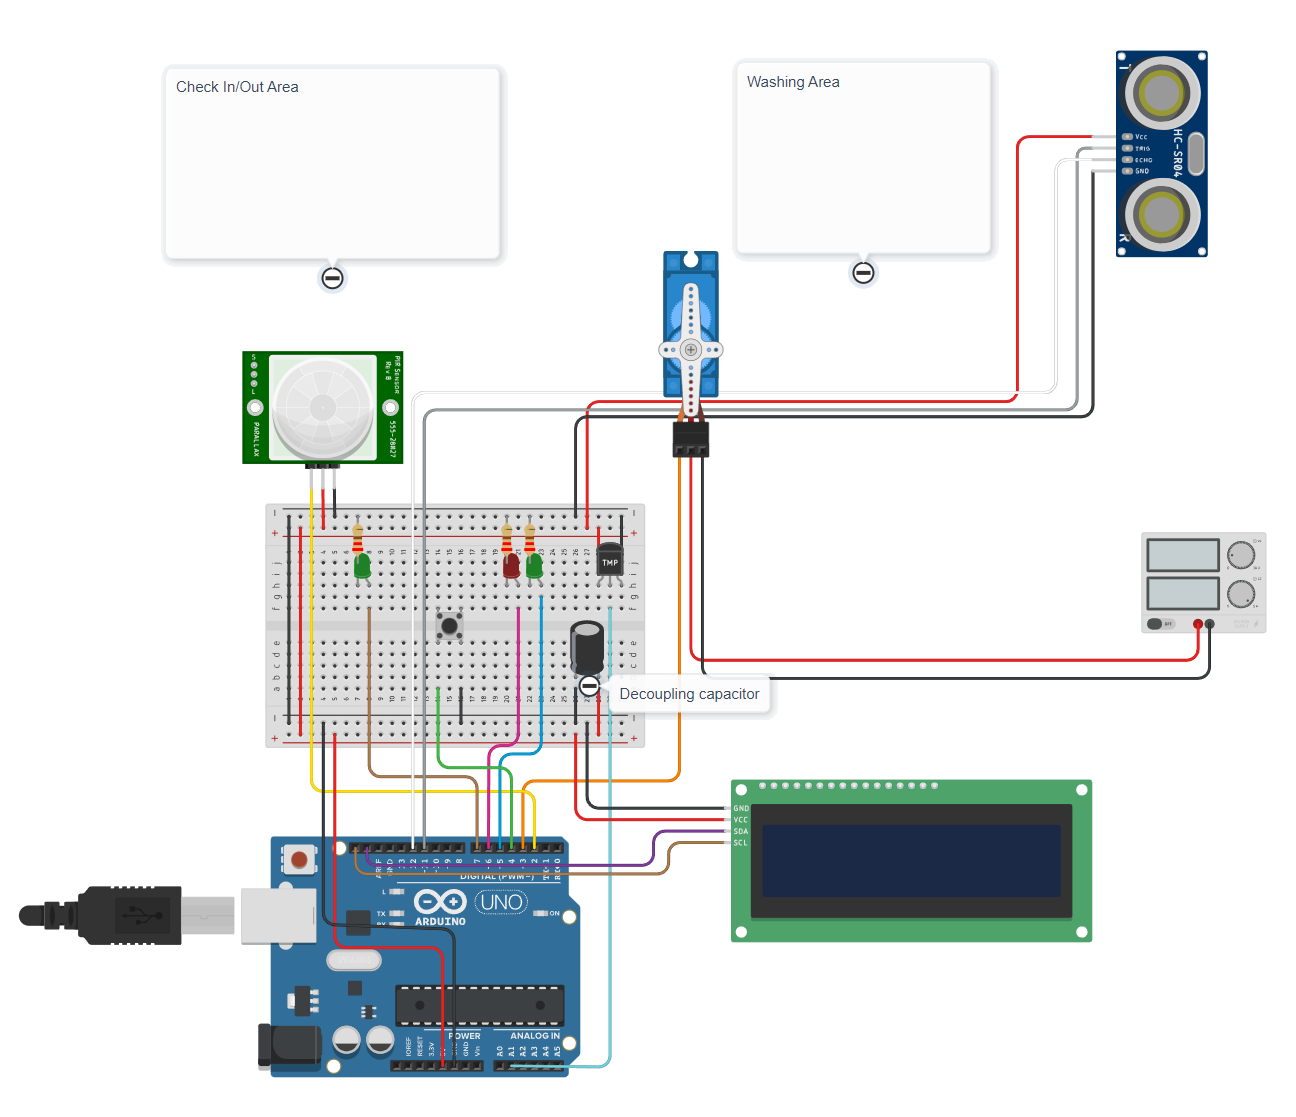
\includegraphics[width=\textwidth]{schematic}
\begin{center}
    \begin{tabular}{|c|c|}
        \hline
        Device             & pinout \\
        \hline
        \hline
        Temperature sensor & A1     \\
        \hline
        Pir                & 2      \\
        \hline
        L1                 & 7      \\
        \hline
        L2                 & 6      \\
        \hline
        L3                 & 5      \\
        \hline
        Servo              & 3      \\
        \hline
        Sonar trig         & 11     \\
        \hline
        Ssonar echo        & 12     \\
        \hline
    \end{tabular}
\end{center}
Since the servo motor might draw more current than the 150mA offered by arduino pins it's advisable to feed the servo with external power.
All the elements attached to the power line create noise that hinder the analog temperature sensor's readings.\\
To dampen this effect it is possible to add decoupling capacitors (10-100 uF) to filter a bit those variation.
\pagebreak


\section{Software Architecture}
\subsection{Arduino}

The program running on arduino is written in C++ using the wiring framework and the platformIo utility.\\
It is managed by a syncronous scheduler, it is triggered by a timer and launches non cooperative tasks.\\
Each task period has been chosen accordingly to its operative requirements, and is a multiple of the base period of the scheduler.
Some empiric tests have been made to ensure that no overrun happens in any scenario.\\
The work tree of the program is divided in:
\begin{itemize}
    \item Sensors, containing interfaces (abstract classes) and implementations for the devices.
    \item actuators, containing interfaces (abstract classes) and implementations for the devices.
    \item System, containing the scheduler and the task interface.
    \item Task, containing all the tasks.
\end{itemize}
On the root are present:
\begin{itemize}
    \item The main file, entry poit of the program, where the scheduler and the tasks are instantiated.
    \item CarWash class, representing the domain of the system with all the shared variables.
    \item Config, configuration file to tune all the parameters of the program.
\end{itemize}
\pagebreak
\subsection{Rust}
The rust application uses "egui", a simple, fast, and highly portable immediate mode GUI library.
The other main crate used is "Serialport" for serial communication, a new thread is created to listen to the selected port,
it expects a \underline{\textbf{Json}} with the parameters of the CarWash class, it then parses it and records the data inside the program.
To do so also mutexes are used to ensure no race conditions since also the gui thread is using the same data.\\
It has been tested both on Windows and MacOs.
\begin{figure}[H]
    \centering
    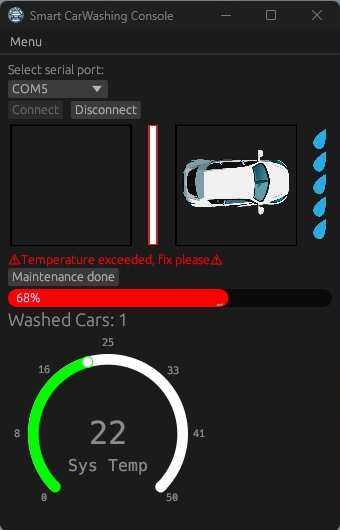
\includegraphics[width=0.50\textwidth]{Dashboard.png}
    \caption{Screenshot of the dashboard ui}
\end{figure}

\pagebreak
\section{General diagram}
\begin{figure}[H]
    \centering
    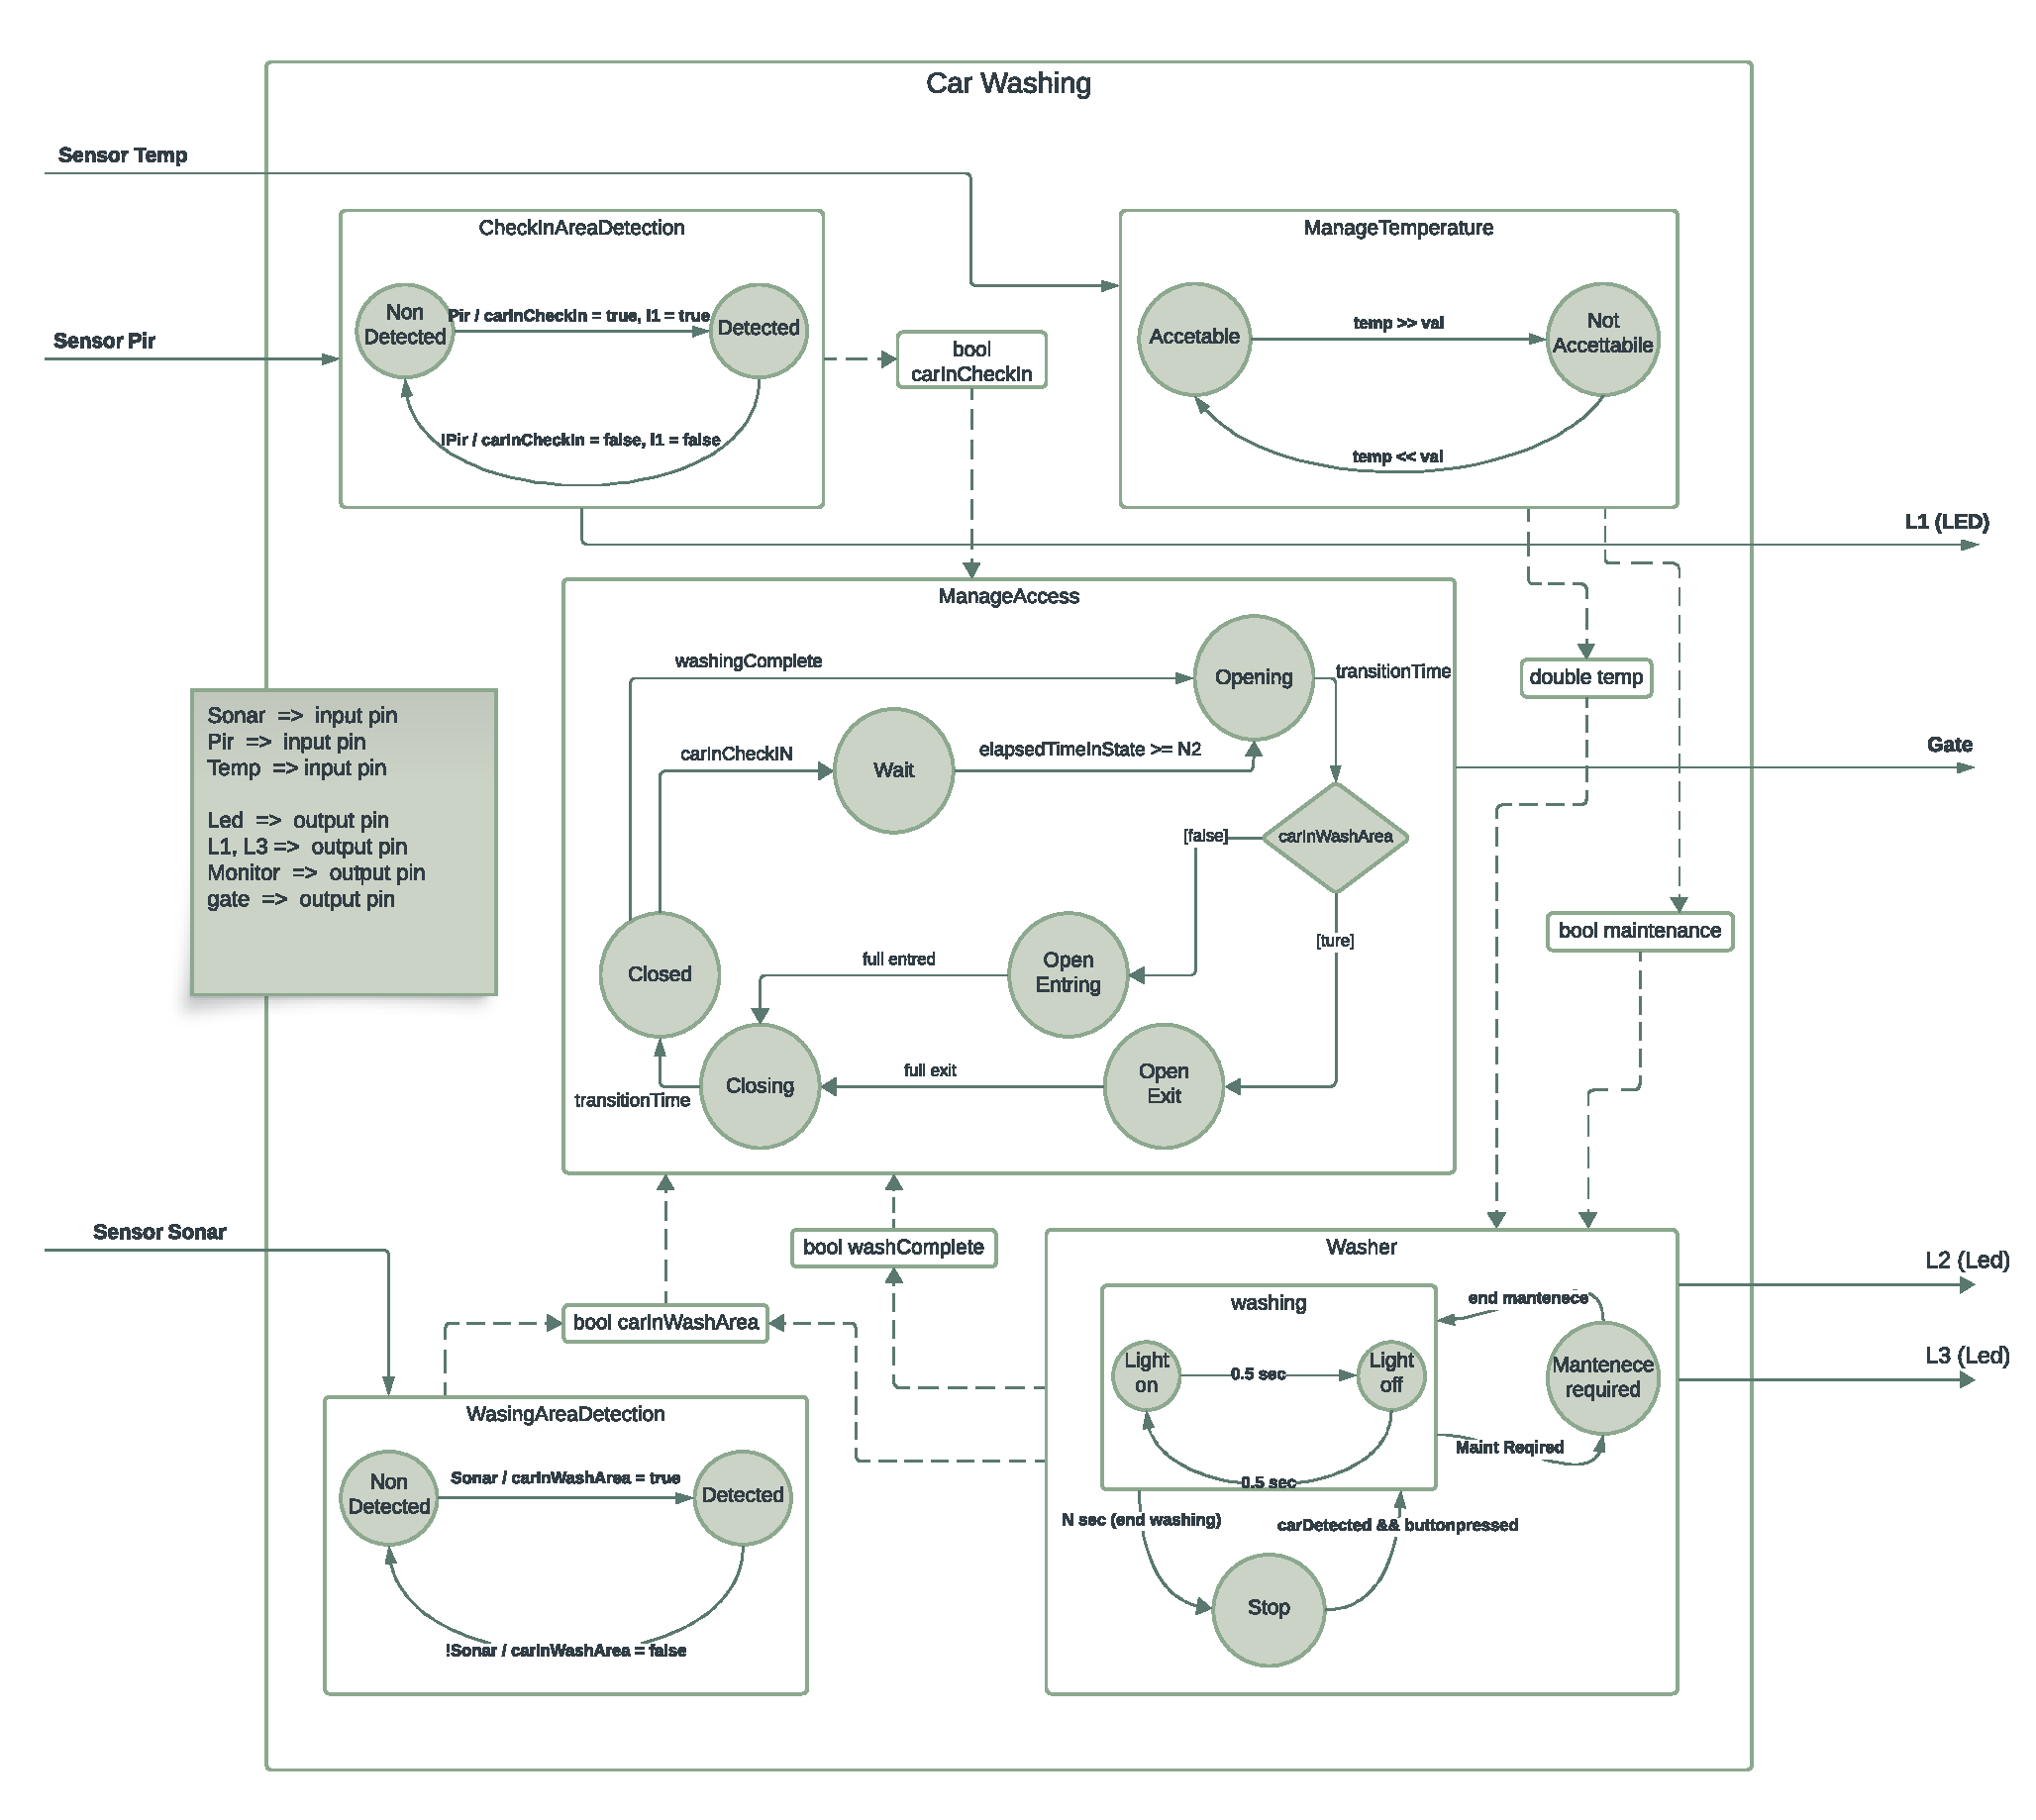
\includegraphics[width=\textwidth]{vertical.pdf}
\end{figure}
\pagebreak
\section{Tasks}
\subsection{checkInDetection}
This task manages the detection of a car inside the check in area with a pir sensor and the state of the L1 led.
\begin{figure}[H]
    \centering
    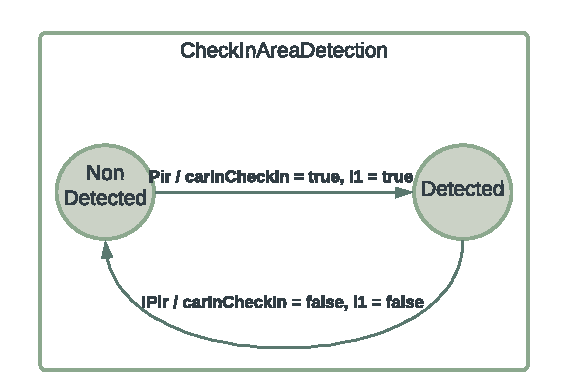
\includegraphics[width=0.7\textwidth]{CheckInAreaDetection.pdf}
\end{figure}
\subsection{washingAreaDetection}
This task manages the detection of a car inside the washing area with a sonar sensor.
\begin{figure}[H]
    \centering
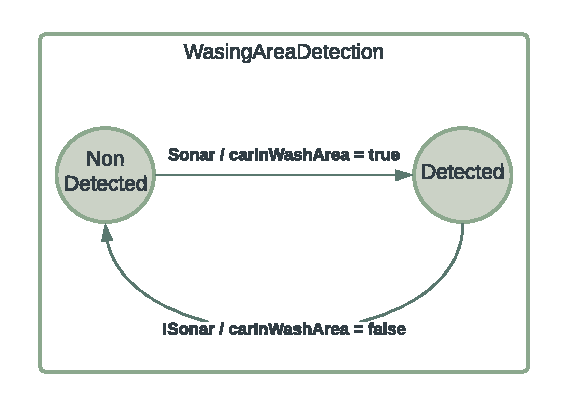
\includegraphics[width=0.7\textwidth]{WashingAreaDetection.pdf}
\end{figure}
\subsection{washer}
This task manages the washing process, L2 and L3 leds.
\begin{figure}[H]
    \centering
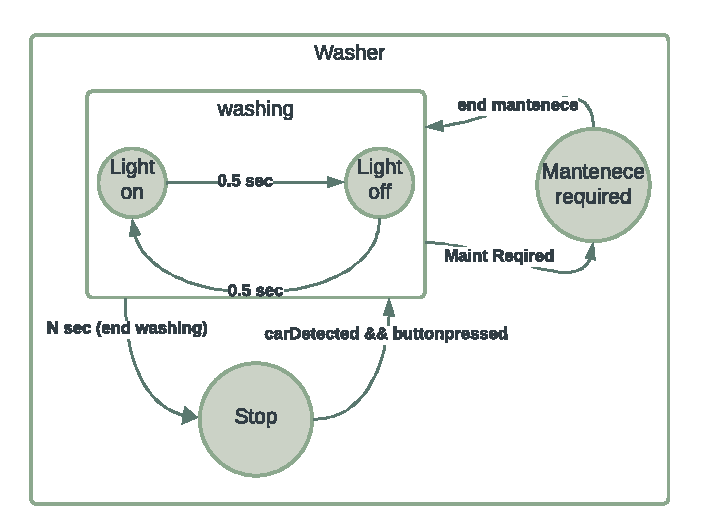
\includegraphics[width=0.8\textwidth]{Washer.pdf}
\end{figure}
\subsection{manageTemperature}
This task checks the temperature with an analog sensor and records it, it also signals if it is over the limit.
\begin{figure}[H]
    \centering
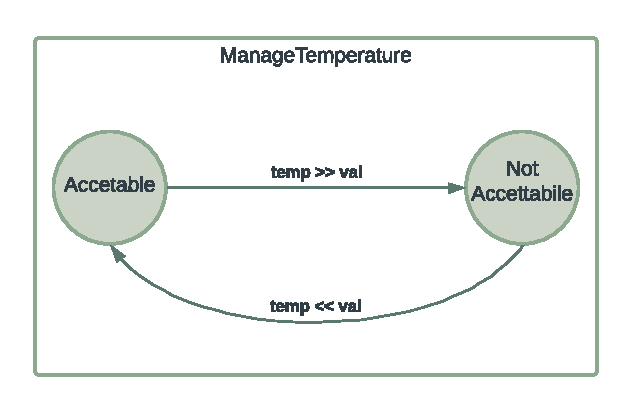
\includegraphics[width=0.8\textwidth]{MangeTemperature.pdf}
\end{figure}
\subsection{manageAccess}
This task manages the position of the bar.
\begin{figure}[H]
    \centering
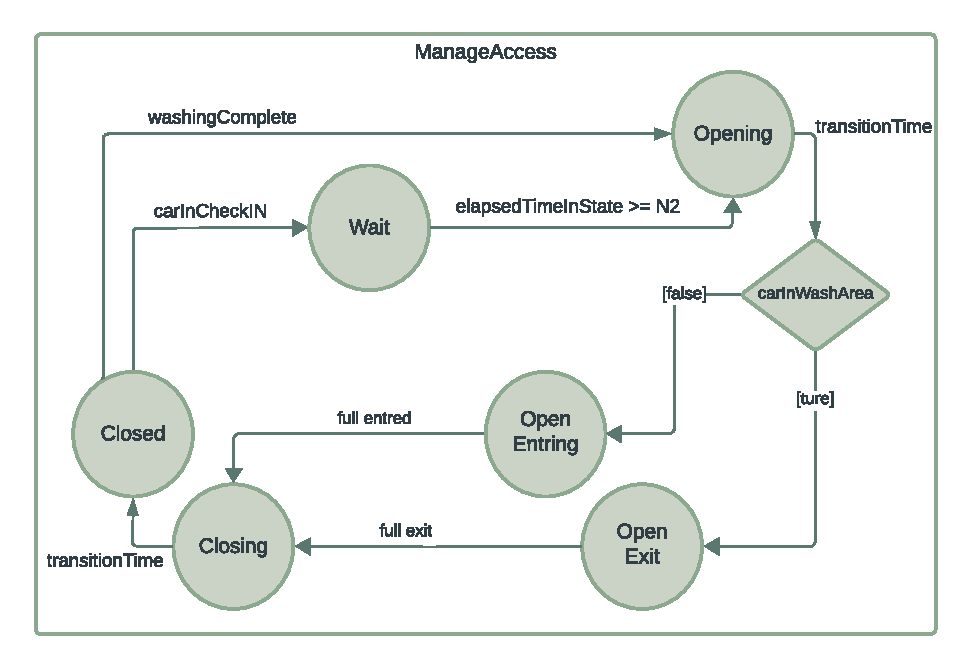
\includegraphics[width=0.8\textwidth]{ManageAccess.pdf}
\end{figure}
\subsection{displayFeedback}
This task displaies the appropriate message on the display.
\subsection{communicator}
This task is responsible of communicating via serial with the dashboard.
\subsection{sleepTask}
This task triggers the sleep when the situation requires it.

